\chapter{METHODOLOGY}
The dataset utilized in this arrangement has been gathered from Kaggle which is “Historical Weather Data for Indian Cities” from which we have chosen the data for “Jhansi City”. The dataset was created by keeping in mind the necessity of such historical weather data in the community. The dataset was used with the help of worldweatheronline.com . The datasets contain  weather data from 01-01-2019 to 01-02-2023. The data of the city is for more than 4 years. This data can be used to visualize the change in data or can be used to predict the weather.
\\
\\
The main target of this dataset can be used to predict the weather for the next day or week with huge amounts of data provided in the dataset.  This data can also be used to make visualizations which would help to understand the impact of global warming over the various aspects of the weather like precipitation, humidity, temperature, etc.
\\
\\
In this project, we are concentrating on the temperature prediction of Jhansi city with the help of various machine learning algorithms and various regressions. By applying various regressions on the historical weather dataset of Jhansi's city we are predicting the temperature like first we are applying Multiple Linear regression, then Neural Network[7].
% table aani hai idhar
\\
\\
\\
\\
\\
\\
\section{Plots(Various Parameters Present in the dataset)}
\begin{figure}[htbp]
     \centering
     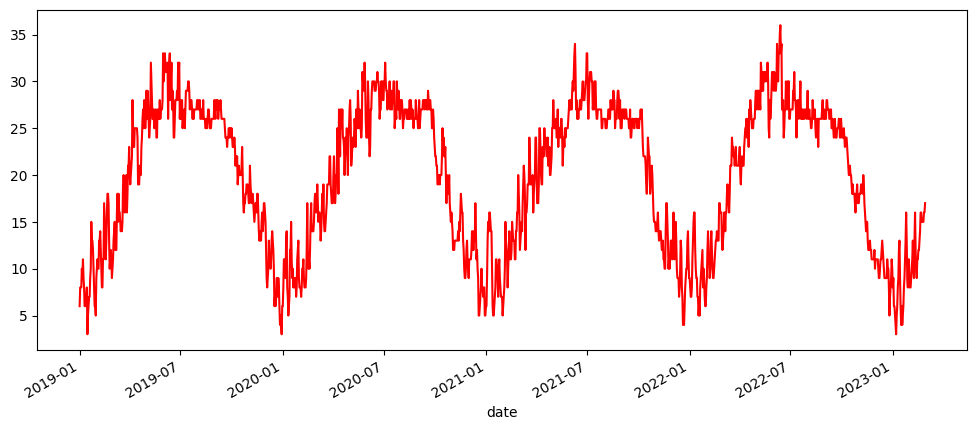
\includegraphics[width=0.8\linewidth]{images/outputs/temp_min.png}
     \caption{ Minimum Temperature Plot}
 \end{figure}
 \begin{figure}[htbp]
     \centering
     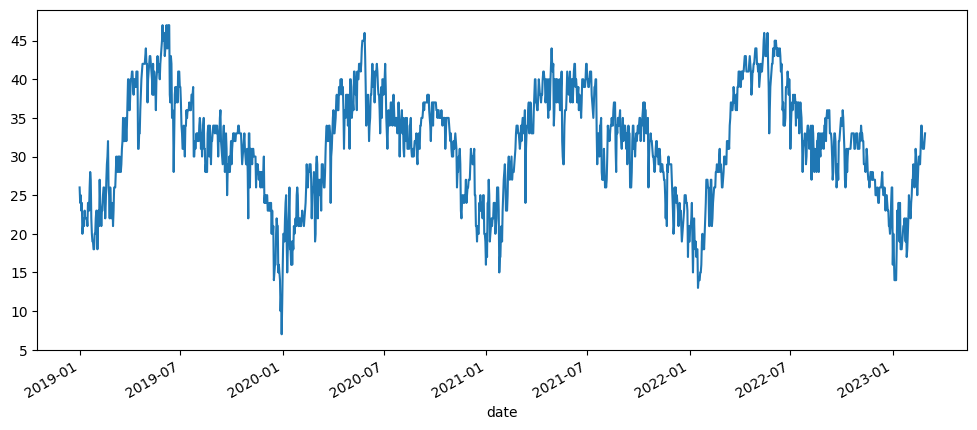
\includegraphics[width=0.8\linewidth]{images/outputs/temp_max.png}
     \caption{ Maximum Temperature Plot}
 \end{figure}
 \begin{figure}
     \centering
     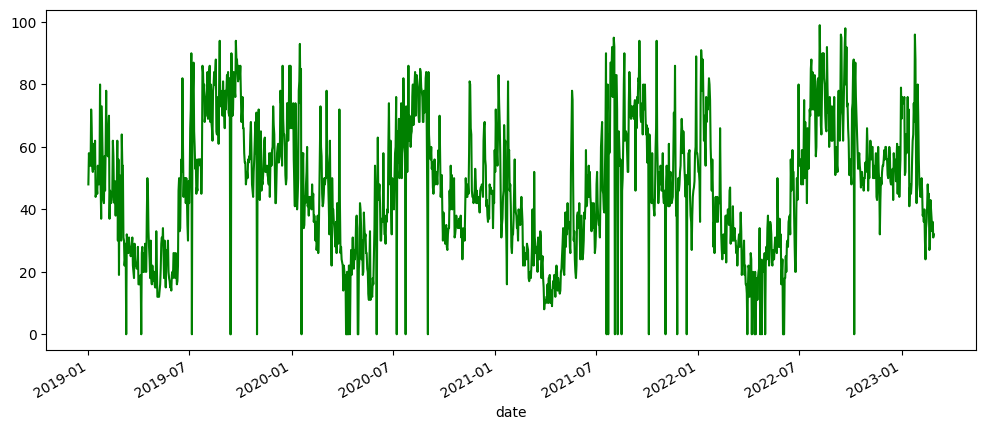
\includegraphics[width=0.8\linewidth]{images/outputs/hum_min.png}
     \caption{ Minimum Humidity Plot}
 \end{figure}
 \begin{figure}[htbp]
     \centering
     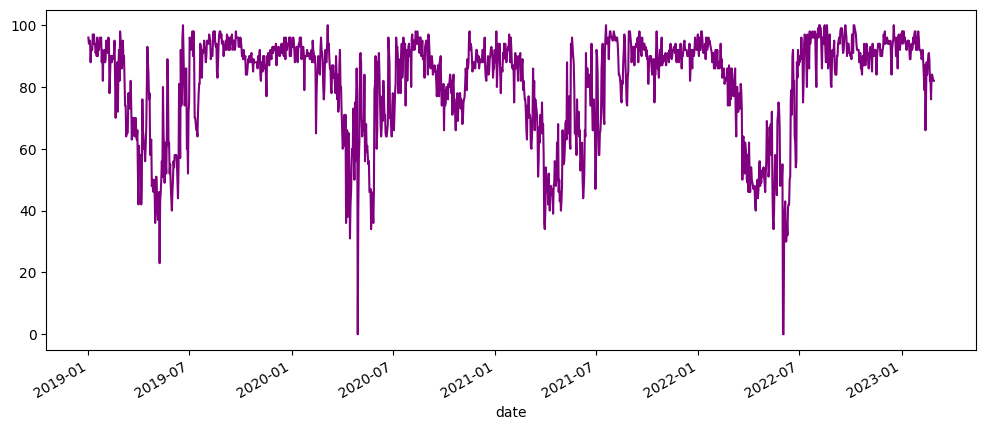
\includegraphics[width=0.8\linewidth]{images/outputs/hum_max.png}
     \caption{ Maximum Humidity Plot}
 \end{figure}
 \begin{figure}[htbp]
     \centering
     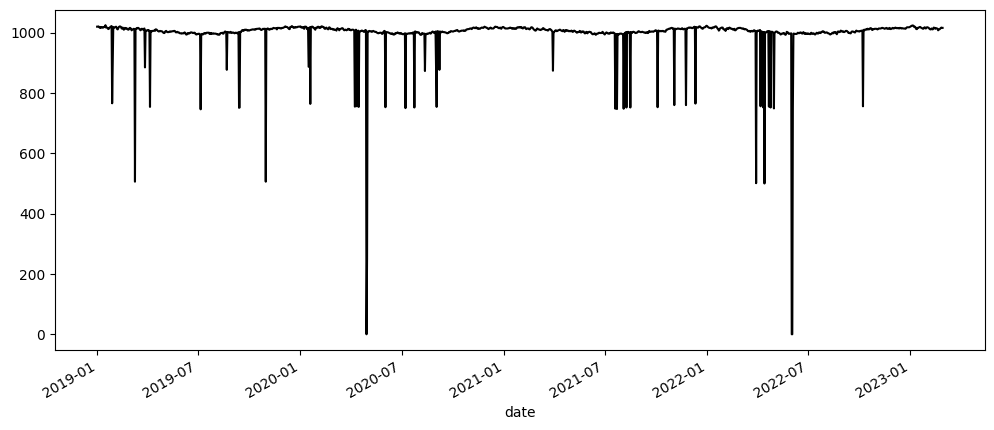
\includegraphics[width=0.8\linewidth]{images/outputs/atm_avg.png}
     \caption{ Average Atmospheric Pressure Plot}
 \end{figure}



